\chapter{Localised bonds: ethane, ethene and ethyne}
\label{ch:localised-bonds}
\index{Localised orbitals}
\index{Hybridisation}
\index{Bond order}
\index{s character}
\index{Pipek-Mezey localisation}
\index{Ethane}\index{Ethene}\index{Ethyne}
\checkedwith{9.5.3-dev}{7e2077af7}
\eccexample{Examples > Organic Chemistry > Bonding in hydrocarbons}
\helppage{localised-orbitals}

Organic chemistry describes ethane, ethene and ethyne with one picture each: four sp$^3$ hybrids on each carbon of ethane, three sp$^2$ hybrids and a p orbital in ethene, two sp hybrids and two p orbitals in ethyne. The orbitals a quantum chemistry program gives are spread over the whole molecule and look nothing like this. ECCE-QM, the program built into ECCE, can turn them into localised orbitals, one for each bond and lone pair, and label each with the hybrid it uses on each atom. This chapter puts the three molecules side by side and asks how well the hybrid picture holds: which bonds ECCE finds, how much s character the carbon hybrids have, and how that goes with the bond lengths, the angles and the stretching frequencies.

\section*{This requires}
Nothing beyond ECCE: the three calculations are in the Organic Chemistry example set. Localised orbitals and their hybrid labels are available only for ECCE-QM calculations.

\section{Background}
A localised orbital describes the same electrons as the orbitals of the calculation, divided up differently. The occupied orbitals are mixed among themselves until each one sits on as few atoms as possible, and what comes out is, for an ordinary closed-shell molecule, one orbital per core, bond and lone pair. The total electron density and the energy do not change; only the bookkeeping does. ECCE-QM uses the criterion of Pipek and Mezey \cite{pipek1989}, which makes each orbital's charge sit on as few atoms as possible. In a planar molecule such as ethene this criterion keeps the $\sigma$ and the $\pi$ bond apart, so the localised orbitals come out in the form organic chemistry draws.

For each localised bond orbital ECCE works out how much of it is s and how much p on each of the two atoms, and writes the ratio as a hybrid label. \texttt{sp3.6} means 3.6 times as much p as s, so the hybrid is $1/(1+3.6) = 22\,\%$ s. The ideal hybrids of the textbook are sp$^3$ (25\,\% s), sp$^2$ (33\,\%) and sp (50\,\%). A hydrogen contributes only its s orbital, written \texttt{s}, and a $\pi$ bond gets no label because it is made of p orbitals across the bond. The labels are worked out from the orbitals and rounded to one decimal, so they describe the bond; they are not a measured quantity.
\index{Hybridisation!s character}

\section{The calculations}
The topic \menu{Bonding in hydrocarbons} has three ECCE-QM calculations made for this comparison, \emph{ethane}, \emph{ethene} and \emph{ethyne}. Each is a geometry optimisation followed by frequencies with B3LYP \cite{becke1993} and the 6-31G* basis \cite{hariharan1973}, with \menu{Localised orbitals} ticked under \menu{Runtype Details}. All three use the same method, so their bond lengths and hybrids can be compared directly.

\section{Procedure}
\begin{enumerate}
	\item In the Organizer, choose \menu{File > Open Example Calculations}, pick \menu{Organic Chemistry} and click \menu{OK}.
	\item In \menu{Examples > Bonding in hydrocarbons}, open \emph{ethane} in the Viewer and choose \menu{Properties > MOs}.
	\item In the box next to \menu{Compute}, choose \menu{Localised MO} instead of \menu{MO}. The table now lists the localised orbitals, with the columns \menu{Bond type}, \menu{Atoms} and \menu{Hybrids} (figure~\ref{fig:lb-table}).
	\item Select the row with \menu{$\sigma$} and \menu{C1-C2} and click \menu{Compute} to draw the orbital; then one of the $\sigma$ C1--H rows.
	\item With \menu{Measure}, measure C1--C2, C1--H3, the angle H3--C1--H4 and the angle H3--C1--C2.
	\item Open \menu{Properties > Vibrational spectra > Vibrational Frequencies} and look at the C--H stretches near 3000~cm$^{-1}$ and above.
	\item Repeat for \emph{ethene} and \emph{ethyne}, and draw their $\pi$ orbitals too.
\end{enumerate}
\index{Localised orbitals!showing}\index{MOs panel!Localised MO}\index{Measure}

\begin{figure}[htbp]
	\centering
	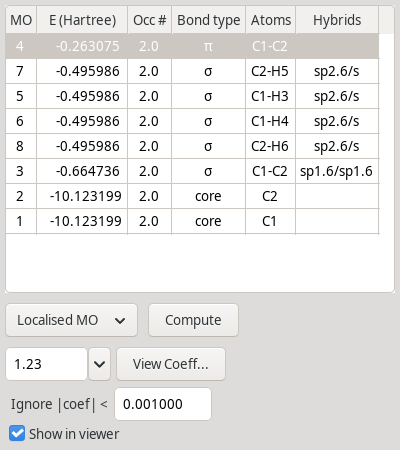
\includegraphics[width=0.5\linewidth]{localised-bonds/loctable-ethene.ecce-9.5.3-dev.png}
	\caption{The localised orbitals of ethene in the \menu{MOs} panel (\menu{Localised MO}). Each row names one core orbital, bond or lone pair, the atoms it belongs to and, for a $\sigma$ bond, the hybrid on each atom.}
	\label{fig:lb-table}
\end{figure}

\section{The bonds ECCE finds}
The localised orbitals come out exactly as the Lewis structures are drawn (table~\ref{tab:lb-orbitals}). Each molecule has two carbon core orbitals and one $\sigma$ orbital for every C--H bond. The C--C bond is one $\sigma$ orbital in ethane, a $\sigma$ and a $\pi$ orbital in ethene, and a $\sigma$ and two $\pi$ orbitals in ethyne. Counting the orbitals between the two carbons gives the bond order, 1, 2 and 3.

\begin{table}[htbp]
	\centering
	\caption{The occupied localised orbitals of the three molecules as the \menu{MOs} panel lists them (B3LYP/6-31G*), with its columns \menu{Bond type}, \menu{Atoms}, \menu{Hybrids} and \menu{E (Hartree)}; orbitals of the same kind are counted together. Every orbital holds two electrons.}
	\label{tab:lb-orbitals}
	\begin{tabular}{lllllr}
		\toprule
		Molecule & Bond type & Atoms & Hybrids & Number & $E$ (hartree) \\
		\midrule
		ethane & core & C1, C2 & & 2 & $-10.125$ \\
		       & $\sigma$ & C1-C2 & sp2.7/sp2.7 & 1 & $-0.517$ \\
		       & $\sigma$ & C-H & sp3.6/s & 6 & $-0.466$ \\
		\midrule
		ethene & core & C1, C2 & & 2 & $-10.123$ \\
		       & $\sigma$ & C1-C2 & sp1.6/sp1.6 & 1 & $-0.665$ \\
		       & $\pi$ & C1-C2 & & 1 & $-0.263$ \\
		       & $\sigma$ & C-H & sp2.6/s & 4 & $-0.496$ \\
		\midrule
		ethyne & core & C1, C2 & & 2 & $-10.104$ \\
		       & $\sigma$ & C1-C2 & sp0.8/sp0.8 & 1 & $-0.807$ \\
		       & $\pi$ & C1-C2 & & 2 & $-0.278$ \\
		       & $\sigma$ & C-H & sp1.4/s & 2 & $-0.568$ \\
		\bottomrule
	\end{tabular}
\end{table}

The pictures (figure~\ref{fig:lb-orbitals}) show what the labels mean. The C--H orbital is a single lobe between the carbon and the hydrogen, with a small tail on the far side of the carbon. The C--C $\sigma$ orbital is symmetric about the C--C axis. The $\pi$ orbital of ethene has two lobes, above and below the plane of the atoms, with a node in that plane. In ethyne the two $\pi$ orbitals are the same shape at right angles to each other, and together they make a cylinder of density around the C--C axis.

\begin{figure}[htbp]
	\centering
	\begin{tabular}{@{}ccc@{}}
		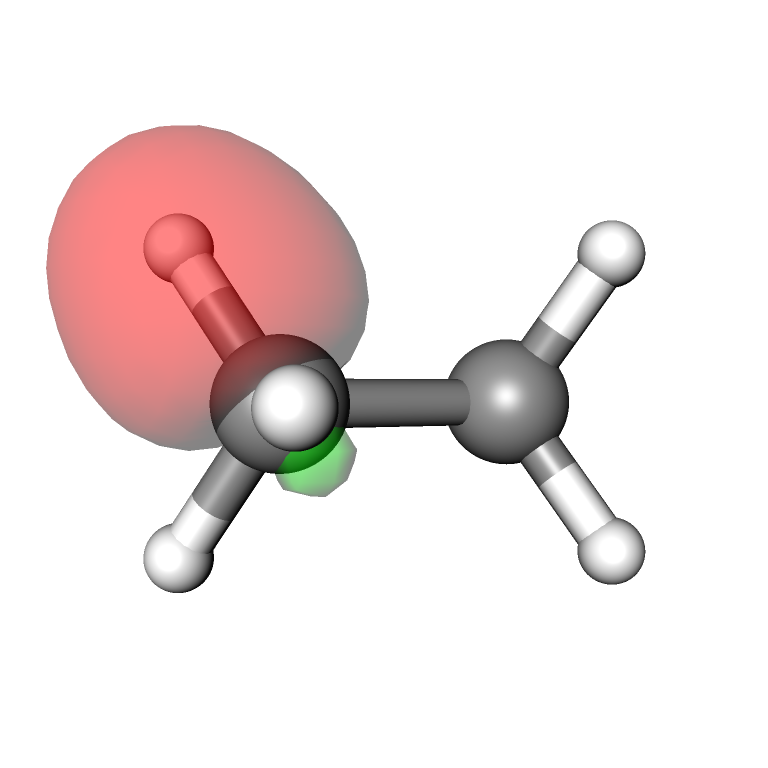
\includegraphics[width=0.31\linewidth]{localised-bonds/ethane-ch-sigma.ecce-9.5.3-dev.png} &
		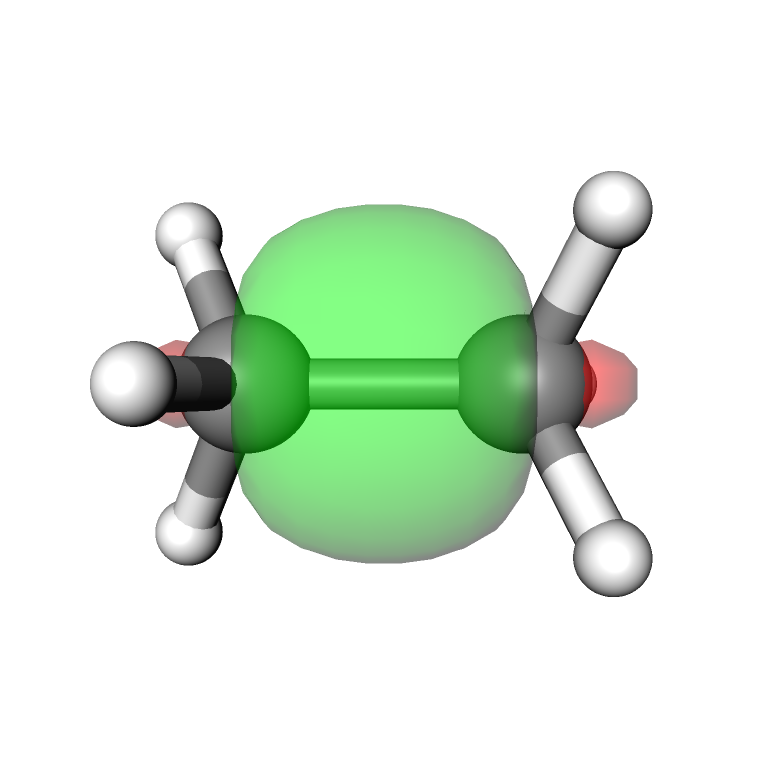
\includegraphics[width=0.31\linewidth]{localised-bonds/ethane-cc-sigma.ecce-9.5.3-dev.png} & \\
		\small ethane, $\sigma$ C--H & \small ethane, $\sigma$ C--C & \\[4pt]
		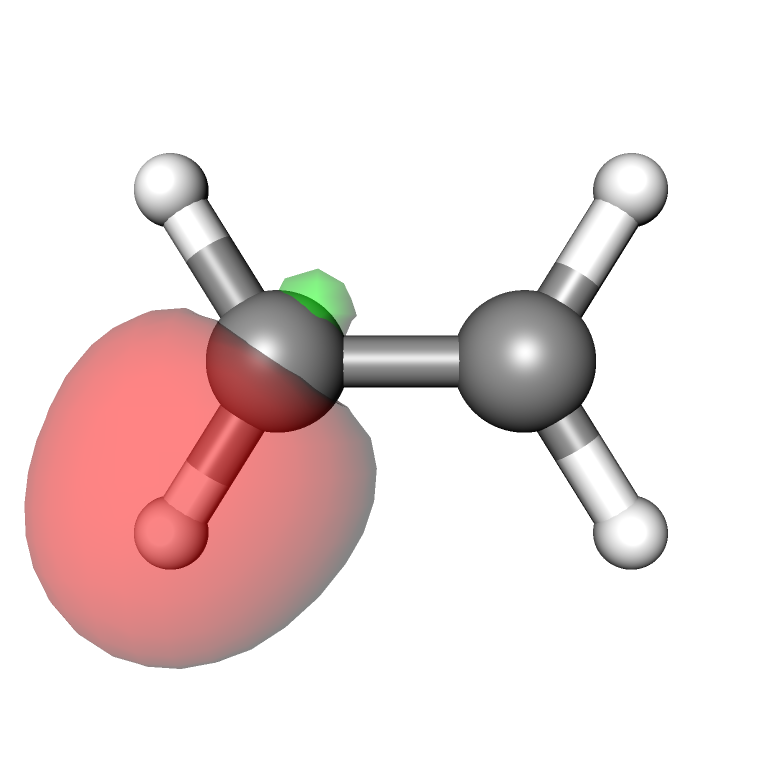
\includegraphics[width=0.31\linewidth]{localised-bonds/ethene-ch-sigma.ecce-9.5.3-dev.png} &
		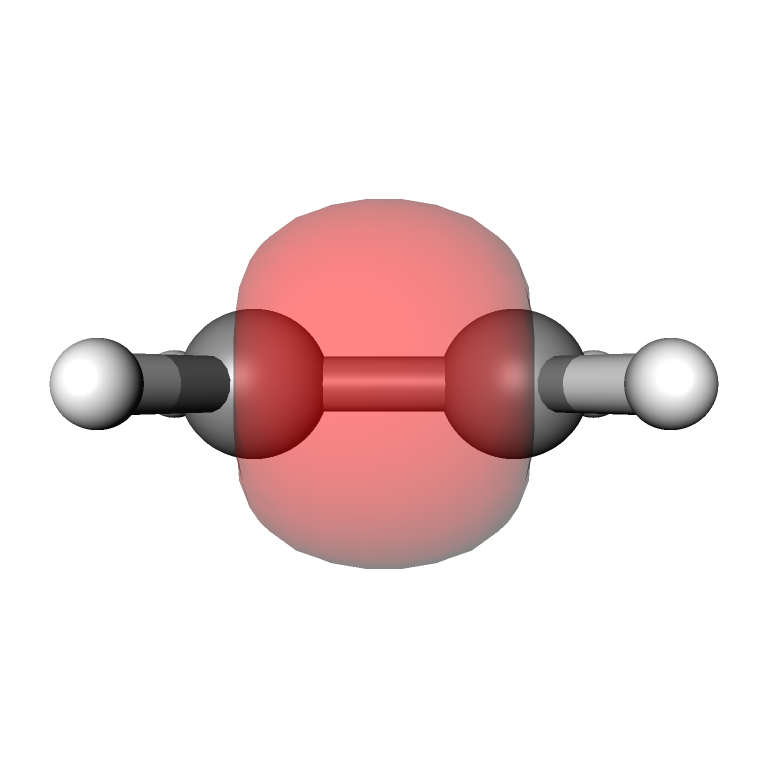
\includegraphics[width=0.31\linewidth]{localised-bonds/ethene-cc-sigma.ecce-9.5.3-dev.png} &
		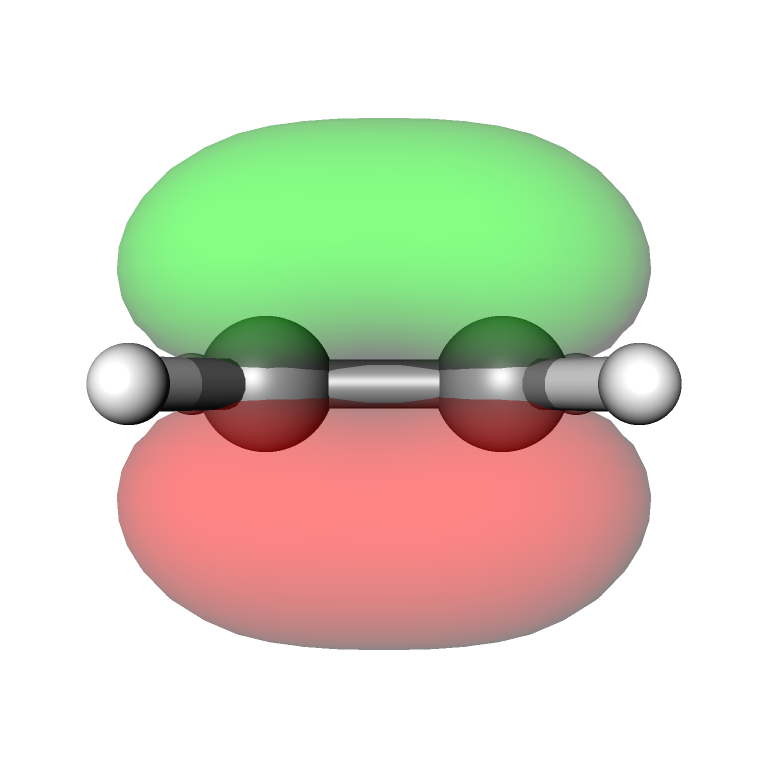
\includegraphics[width=0.31\linewidth]{localised-bonds/ethene-cc-pi.ecce-9.5.3-dev.png} \\
		\small ethene, $\sigma$ C--H & \small ethene, $\sigma$ C--C & \small ethene, $\pi$ C--C \\[4pt]
		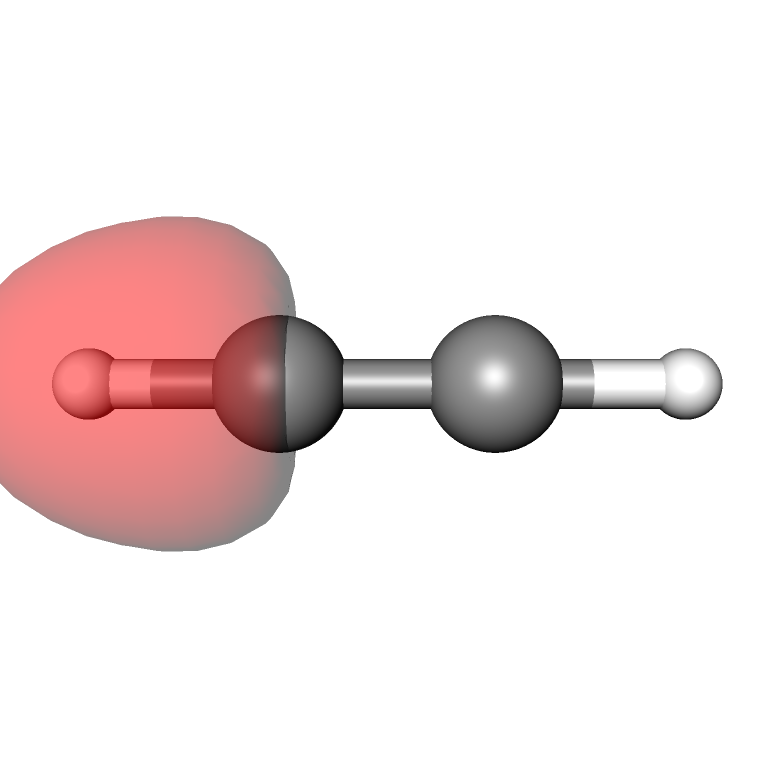
\includegraphics[width=0.31\linewidth]{localised-bonds/ethyne-ch-sigma.ecce-9.5.3-dev.png} &
		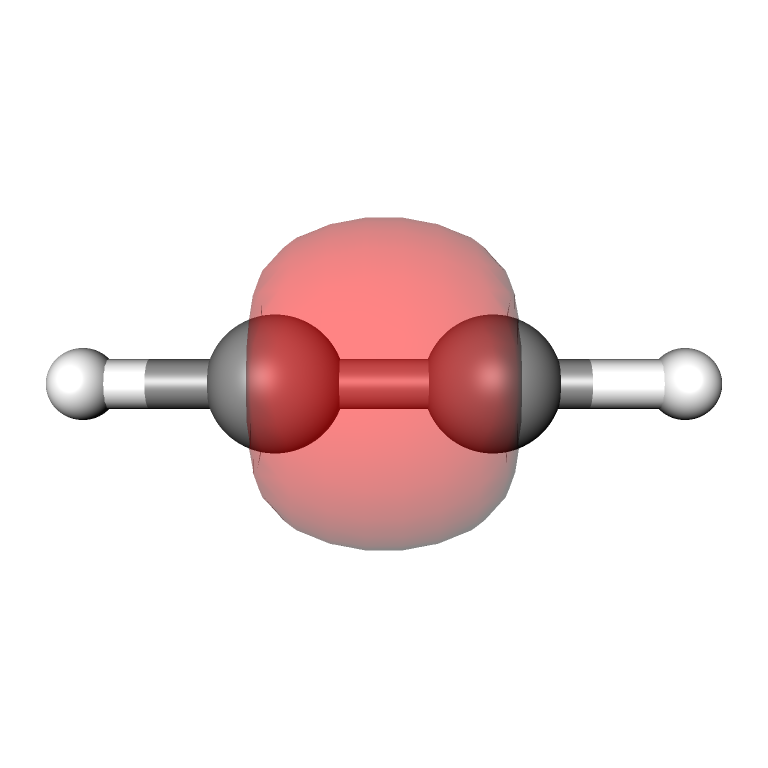
\includegraphics[width=0.31\linewidth]{localised-bonds/ethyne-cc-sigma.ecce-9.5.3-dev.png} &
		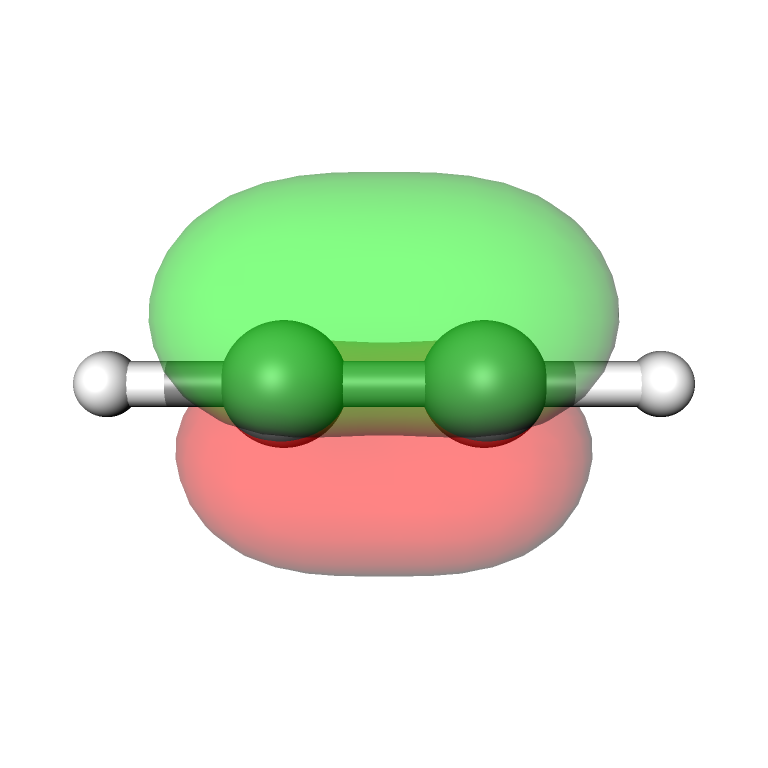
\includegraphics[width=0.31\linewidth]{localised-bonds/ethyne-cc-pi1.ecce-9.5.3-dev.png} \\
		\small ethyne, $\sigma$ C--H & \small ethyne, $\sigma$ C--C & \small ethyne, one of the two $\pi$ \\
	\end{tabular}
	\caption{Localised orbitals of ethane, ethene and ethyne drawn by the \menu{MOs} panel (\menu{Localised MO}, default isovalue; the two colours are the two signs of the orbital). Each molecule is shown with its C--C axis across the page.}
	\label{fig:lb-orbitals}
\end{figure}

\section{Hybrids and s character}
Table~\ref{tab:lb-trends} collects the hybrid labels with the geometry and the stretching frequencies. On carbon, the s character of both kinds of $\sigma$ bond rises from ethane to ethene to ethyne: in the C--H bond from 22 to 28 to 42\,\%, in the C--C bond from 27 to 38 to 56\,\%. The trend is the one the textbook names, sp$^3$, sp$^2$, sp, but the numbers are not the ideal 25, 33 and 50\,\%. In each molecule the carbon puts more s character into the bond to the other carbon than into its bonds to hydrogen, so that even in ethane the four bonds of a carbon are not four identical sp$^3$ hybrids. In ethene and ethyne the $\pi$ bonds take p orbitals only, which leaves the s orbital of carbon to the $\sigma$ bonds; that is why the $\sigma$ hybrids of the multiple bonds are so rich in s.

The hybrids explain the angles. An sp$^3$ carbon has its bonds at the tetrahedral angle, \ang{109.5}; ethane comes close, with H--C--H \ang{107.5} and H--C--C \ang{111.3}. The H--C--H angle in ethene, \ang{116.3}, is a few degrees below the \ang{120} of three equal sp$^2$ hybrids, and H--C--C opens to \ang{121.9}, as the carbon with more s character towards the other carbon would make it. Ethyne is linear.
\index{Bond angles!hybridisation}

\begin{table}[htbp]
	\centering
	\caption{Hybrids, geometry and stretching frequencies of the three molecules (ECCE-QM, B3LYP/6-31G*, optimised geometries). Hybrid labels from the \menu{MOs} panel; s character on carbon is $1/(1+n)$ for a label sp$n$. Lengths and angles from the optimised structures, frequencies from \menu{Vibrational Frequencies} (harmonic, not scaled).}
	\label{tab:lb-trends}
	\begin{tabular}{lrrr}
		\toprule
		 & ethane & ethene & ethyne \\
		\midrule
		C--C bond order & 1 & 2 & 3 \\
		C--C $\sigma$ hybrid on C & sp2.7 & sp1.6 & sp0.8 \\
		\quad s character & 27\,\% & 38\,\% & 56\,\% \\
		C--H $\sigma$ hybrid on C & sp3.6 & sp2.6 & sp1.4 \\
		\quad s character & 22\,\% & 28\,\% & 42\,\% \\
		\midrule
		C--C (\AA) & 1.531 & 1.332 & 1.205 \\
		C--H (\AA) & 1.097 & 1.088 & 1.067 \\
		H--C--H & \ang{107.5} & \ang{116.3} & -- \\
		H--C--C & \ang{111.3} & \ang{121.9} & \ang{180.0} \\
		\midrule
		C--C stretch (cm$^{-1}$) & 1009 & 1719 & 2086 \\
		C--H stretches (cm$^{-1}$) & 3045--3120 & 3149--3245 & 3440, 3540 \\
		\bottomrule
	\end{tabular}
\end{table}

\section{Bond lengths and stretching frequencies}
The C--C bond shortens from \SI{1.531}{\angstrom} in ethane to \SI{1.332}{\angstrom} in ethene and \SI{1.205}{\angstrom} in ethyne, and its stretch moves up from 1009 to 1719 and 2086~cm$^{-1}$ (all three are the totally symmetric C--C stretch, which is not IR active in these molecules). Both follow the bond order, the number of localised orbitals between the carbons.

The C--H bond changes much less, but in the same direction: \SI{1.097}{\angstrom}, \SI{1.088}{\angstrom} and \SI{1.067}{\angstrom}. Here the bond order is one in all three molecules, and what changes is the carbon hybrid. A hybrid with more s character holds its electrons closer to the carbon nucleus, so the bond is shorter and stiffer, and the C--H stretches rise from 3045--3120~cm$^{-1}$ in ethane to 3149--3245 in ethene and 3440 and 3540~cm$^{-1}$ in ethyne. The energies of the localised C--H orbitals in table~\ref{tab:lb-orbitals} fall in the same order, from $-0.466$ to $-0.496$ to $-0.568$~hartree: the electrons of the C--H bond are held more tightly as the s character rises.
\index{Bond length!s character}\index{Infrared spectrum!C--H stretch}

\section{What the labels do not say}
The s shares of the four $\sigma$ bonds of a carbon add up to 0.92 in ethane ($3 \times 0.217 + 0.270$), 0.94 in ethene and 0.97 in ethyne, close to one 2s orbital but not exactly one. Each label is worked out from its own orbital, leaves out the small contribution of the d functions of the basis set and is rounded to one decimal. The labels should be read as a trend between molecules and between bonds, with an uncertainty of a few per cent, rather than as exact compositions.

\section{In class}
Start from the Lewis structures and ask what each line stands for; the \menu{Localised MO} table answers with one orbital per line, and the $\pi$ orbitals of ethene and ethyne are the second and third lines of the multiple bonds. The table of hybrids is then a test of the sp$^3$/sp$^2$/sp picture: the order is right, the numbers are not the ideal ones, and the difference between the C--C and the C--H hybrids of the same carbon is the point where the simple picture needs refining. The C--H bond length and the C--H stretch tie the hybrid to things that can be measured; the high C--H stretch of ethyne is the band by which a terminal alkyne is recognised in an infrared spectrum.

\section{History}
Pauling \cite{pauling1931} and Slater \cite{slater1931} introduced hybrid orbitals in 1931 to explain why carbon forms four equivalent bonds at the tetrahedral angle when its valence orbitals are one 2s and three 2p orbitals. The first systematic ways to turn the delocalised orbitals of a calculation into localised ones came three decades later: Foster and Boys made each orbital as compact in space as possible \cite{foster1960}, and Edmiston and Ruedenberg maximised the repulsion of the electrons within each orbital \cite{edmiston1963}. Both criteria give a double bond as two equivalent bent bonds rather than a $\sigma$ and a $\pi$ bond. Pipek and Mezey's criterion, which counts how many atoms an orbital's charge is spread over \cite{pipek1989}, keeps $\sigma$ and $\pi$ apart and gives the description used in this chapter.
\index{Pauling, Linus}\index{Slater, John C.}\index{Boys, S. Francis}\index{Edmiston, Clyde}\index{Ruedenberg, Klaus}\index{Pipek, J\'anos}\index{Mezey, Paul G.}
